%%%%%%%%%%%%%%%%%%%%%%%%%%%%%%%%%%%%%%%%%
% baposter Landscape Poster
% LaTeX Template
% Version 1.0 (11/06/13)
%
% baposter Class Created by:
% Brian Amberg (baposter@brian-amberg.de)
%
% This template has been downloaded from:
% http://www.LaTeXTemplates.com
%
% License:
% CC BY-NC-SA 3.0 (http://creativecommons.org/licenses/by-nc-sa/3.0/)
%
%%%%%%%%%%%%%%%%%%%%%%%%%%%%%%%%%%%%%%%%%

% \title{CSAFE poster template}

%-------------------------------------------------------------------------
%	PACKAGES AND OTHER DOCUMENT CONFIGURATIONS
%-------------------------------------------------------------------------

\documentclass[landscape,a0paper,fontscale=0.25, margin = 25mm]{baposter} % Adjust the font scale/size here

\usepackage{graphicx} % Required for including images
\graphicspath{{figures/}} % Directory in which figures are stored

\usepackage{amsmath} % For typesetting math
\usepackage{amssymb} % Adds new symbols to be used in math mode

\usepackage{booktabs} % Top and bottom rules for tables
\usepackage{enumitem} % Used to reduce itemize/enumerate spacing
\usepackage{palatino} % Use the Palatino font

\usepackage{natbib}

\usepackage[font=small,labelfont=bf]{caption} % Required for specifying captions to tables and figures

\usepackage{subcaption}
\usepackage{tabu}
\usepackage{enumitem} % Itemize separation
\setlist{nosep} % or \setlist{noitemsep} to leave space around whole list
\setitemize{nolistsep,leftmargin=*}

\usepackage{multicol} % Required for multiple columns
\setlength{\columnsep}{1.5em} % Slightly increase the space between columns
\setlength{\columnseprule}{0mm} % No horizontal rule between columns

\usepackage{tikz} % Required for flow chart
\usetikzlibrary{shapes,arrows} % Tikz libraries required for the flow chart in the template

\newcommand{\compresslist}{ % Define a command to reduce spacing within itemize/enumerate environments, this is used right after \begin{itemize} or \begin{enumerate}
\setlength{\itemsep}{1pt}
\setlength{\parskip}{0pt}
\setlength{\parsep}{0pt}
}

\definecolor{lightblue}{rgb}{0,0,0.4} % Defines the color used for content box headers
\definecolor{navyblue}{rgb}{0,0,0.4} % Defines the color used for content box headers
\definecolor{antiquefuchsia}{rgb}{0.57, 0.36, 0.51}
\definecolor{bananayellow}{rgb}{1.0, 0.88, 0.21}
\definecolor{bittersweet}{rgb}{1.0, 0.44, 0.37}
\definecolor{raspberry}{rgb}{0.89, 0.04, 0.36}

% This removes any blank page added in the beginning of a document
\usepackage{atbegshi}% http://ctan.org/pkg/atbegshi
\AtBeginDocument{\AtBeginShipoutNext{\AtBeginShipoutDiscard}}

\usepackage{hyperref}
\renewcommand{\figurename}{Fig.} % Shorten figure caption label
\begin{document}

\begin{poster}
{
%grid=true,
columns=3,
headerborder=closed, % Adds a border around the header of content boxes
colspacing=1em, % Column spacing
bgColorOne=white, % Background color for the gradient on the left side of the poster
bgColorTwo=white, % Background color for the gradient on the right side of the poster
borderColor=lightblue, % Border color
headerColorOne=navyblue, % Background color for the header in the content boxes (left side)
headerColorTwo=lightblue, % Background color for the header in the content boxes (right side)
headerFontColor=white, % Text color for the header text in the content boxes
boxColorOne=white, % Background color of the content boxes
textborder=rectangle, % Format of the border around content boxes, can be: none, bars, coils, triangles, rectangle, rounded, roundedsmall, roundedright, roundedleft, or faded
eyecatcher=true, % Set to false for ignoring the left logo in the title and move the title left
headerheight=0.14\textheight, % Height of the header
headershape=rectangle, % Specify the rounded corner in the content box headers, can be: rectangle, small-rounded, roundedright, roundedleft or rounded
headerfont=\Large\bf, % Large, bold and sans serif font in the headers of content boxes
%textfont={\setlength{\parindent}{1.5em}}, % Uncomment for paragraph indentation
linewidth=2pt % Width of the border lines around content boxes
}
%-------------------------------------------------------------------------------
%	TITLE SECTION
%-------------------------------------------------------------------------------
%
{
\includegraphics[height=7em]{logo.png}} % First university/lab logo on the left
{\bf{Automatic\ \ Identification\ \ of\ \ Footwear\\\ \ Class\ \  Characteristics}\vspace{0.3em}} % Poster title
{{Miranda Tilton and Dr. Susan VanderPlas, Iowa State University}\vspace*{-0.6em}} % Author names and institution
{
\includegraphics[height=5em]{logo-NIST.jpg}} % Second university/lab logo on the right

%---------------------------------------------------------------------------------
%	OBJECTIVES
%---------------------------------------------------------------------------------

\headerbox{Problem and Objectives}{name=objectives,column=0,row=0,boxpadding=2mm}{

\textbf{Goal:} To automatically identify class characteristics of footwear outsole images.\\
\textbf{Background:} In shoe print analysis, it is often useful to determine the frequency of a given shoe print (or features of the print) in a local population. Machine learning tools, such as neural networks, are an inexpensive and efficient way to automatically identify these features, which may inform about the prevalence of such features.
%\vspace{0.3em} % When there are two boxes, some whitespace may need to be added if the one on the right has more content
}

%----------------------------------------------------------------------------------------
%	Class Characteristics
%----------------------------------------------------------------------------------------

\headerbox{Class Characteristics}{name=classchars,column=0,below=objectives,above=bottom,boxpadding=2mm}{ % This block's bottom aligns with the bottom of the references block

Footwear class characteristics include the size and shape of geometric design elements. Size, orientation, and position of geometric elements are capable of distinguishing most shoes collected in samples from the general population \cite{hancockInterpretationShoeprintComparison2012}, and can be used to speed up database searches for candidate shoe models \cite{pavlouAutomaticExtractionClassification2006}.

\setlength{\tabcolsep}{3.5pt}
\begin{minipage}{\linewidth}
\centering
\tabulinesep=1mm
\begin{tabu}{rlll}
     Bowtie & \raisebox{-.5\height}{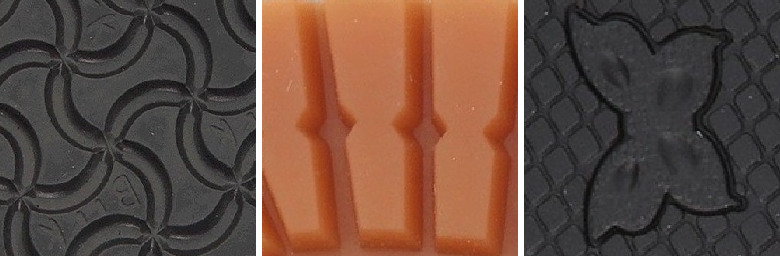
\includegraphics[width=.3\linewidth]{class_examples/bowtie_examples.png}} &
     \raisebox{-.5\height}{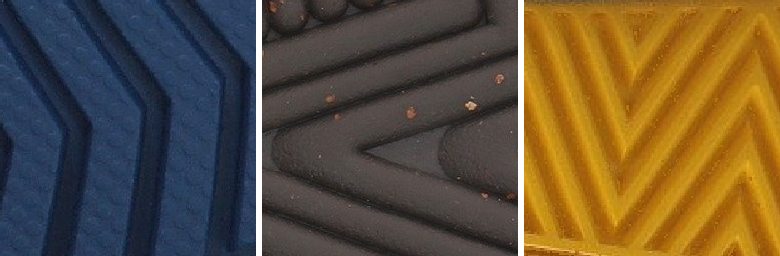
\includegraphics[width=.3\linewidth]{class_examples/chevron_examples.png}} & Chevron \\
     Circle & \raisebox{-.5\height}{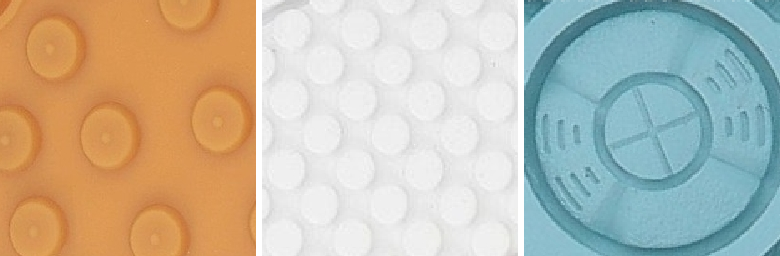
\includegraphics[width=0.3\linewidth]{class_examples/circle_examples.png}} &
     \raisebox{-.5\height}{
\includegraphics[width=0.3\linewidth]{class_examples/line_examples.png}} & Line \\
     Polygon & \raisebox{-.5\height}{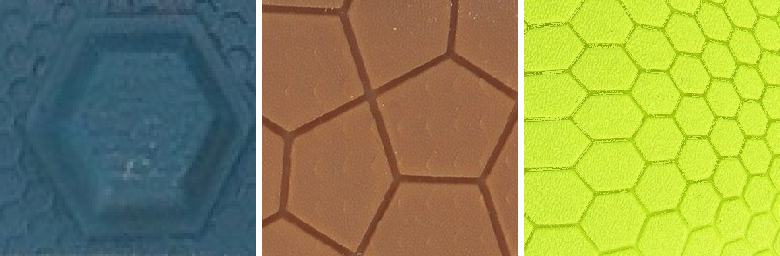
\includegraphics[width=0.3\linewidth]{class_examples/polygon_examples.png}} &
     \raisebox{-.5\height}{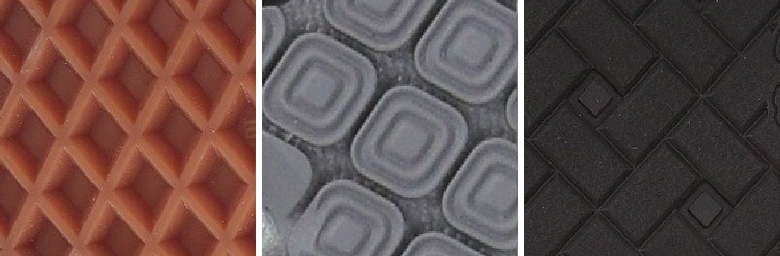
\includegraphics[width=0.3\linewidth]{class_examples/quad_examples.png}} & Quad \\
     Star & \raisebox{-.5\height}{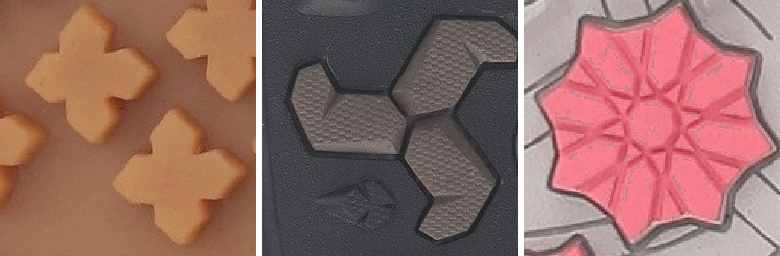
\includegraphics[width=0.3\linewidth]{class_examples/star_examples.png}} &
     \raisebox{-.5\height}{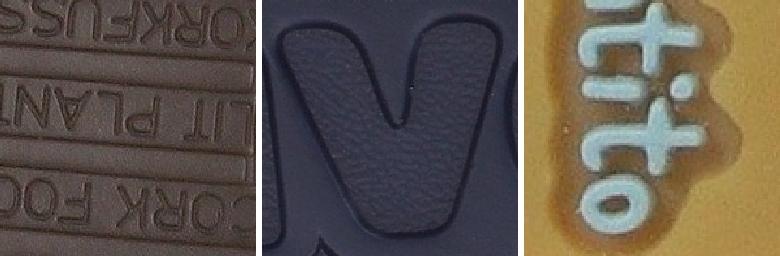
\includegraphics[width=0.3\linewidth]{class_examples/text_examples.png}} & Text \\
     Triangle & \raisebox{-.5\height}{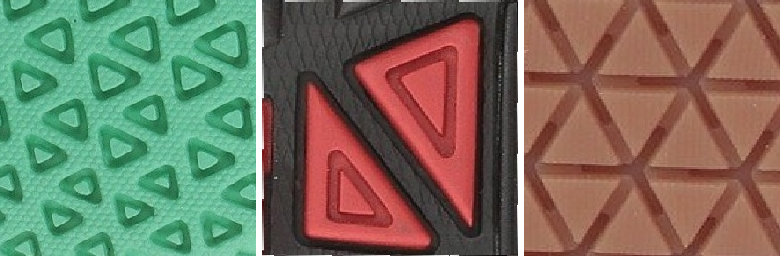
\includegraphics[width=0.3\linewidth]{class_examples/triangle_examples.png}} &
      \raisebox{-.5\height}{} & \\
\end{tabu}
\label{tab:classchars}
\captionof{table}{Geometric Elements. Categories modified from \cite{grossVariabilitySignificanceClass2013}}
\end{minipage}

\vspace{3.5pt}

An automated algorithm which can identify these features in shoe images could be used to assemble an open-access database of shoe models searchable by image upload or feature selection. Spatial relationships between geometric features could be added to further reduce the number of shoes with the same characteristics.

}

%----------------------------------------------------------------------------------------
%	CNNs
%----------------------------------------------------------------------------------------

\headerbox{Convolutional Neural Networks}{name=cnn,column=1,row=0,boxpadding=2mm}{ % This block's bottom aligns with the bottom of the poster
\begin{itemize}\compresslist
    \item A convolutional neural network (CNN) is a tool for deep learning that is well-suited to image analysis.
    \item Inspired by the brain, CNNs learn global patterns using a hierarchy of local feature detection and pooling
    \item VGG16 is a CNN \cite{vgg16} pre-trained on ImageNet, an image database with more than 14 million images spanning 20,000+ categories \cite{ILSVRC15}.
\end{itemize}

\begin{center}
\hfill\mbox{\tiny{Image source: \url{https://bit.ly/2AmjF6K}}}
\vspace{-24pt}
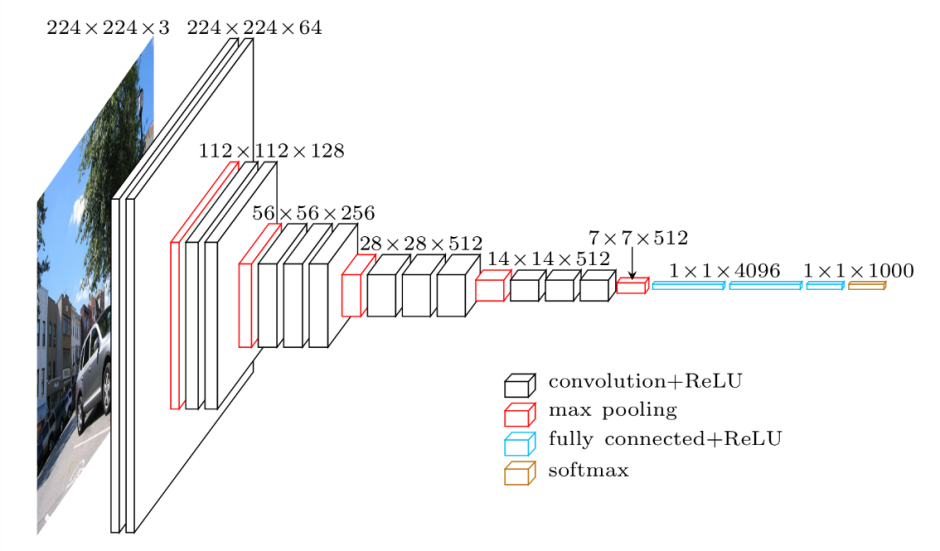
\includegraphics[width=0.9\linewidth]{vgg16.png}
\captionof{figure}{Architecture of VGG16}
\end{center}
\vspace{3pt}
}

%----------------------------------------------------------------------------------------
%	DATA STRUCTURE
%----------------------------------------------------------------------------------------

\headerbox{Data}{name=datastructure,column=1,below=cnn,above=bottom,boxpadding=2mm}{
\begin{minipage}{\linewidth}
\begin{subfigure}[b]{.45\linewidth}
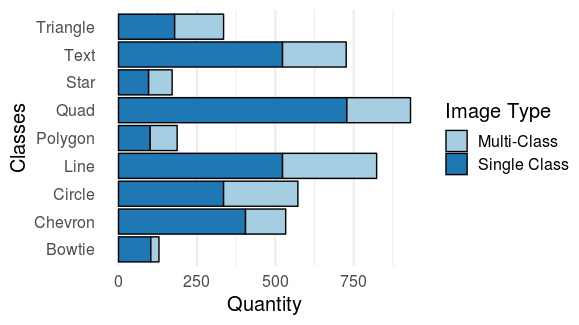
\includegraphics[width=\linewidth]{quantity_bars_horiz.png}
\captionof{figure}{Label Frequency}
\end{subfigure}\hfill
\begin{subfigure}[b]{.45\linewidth}
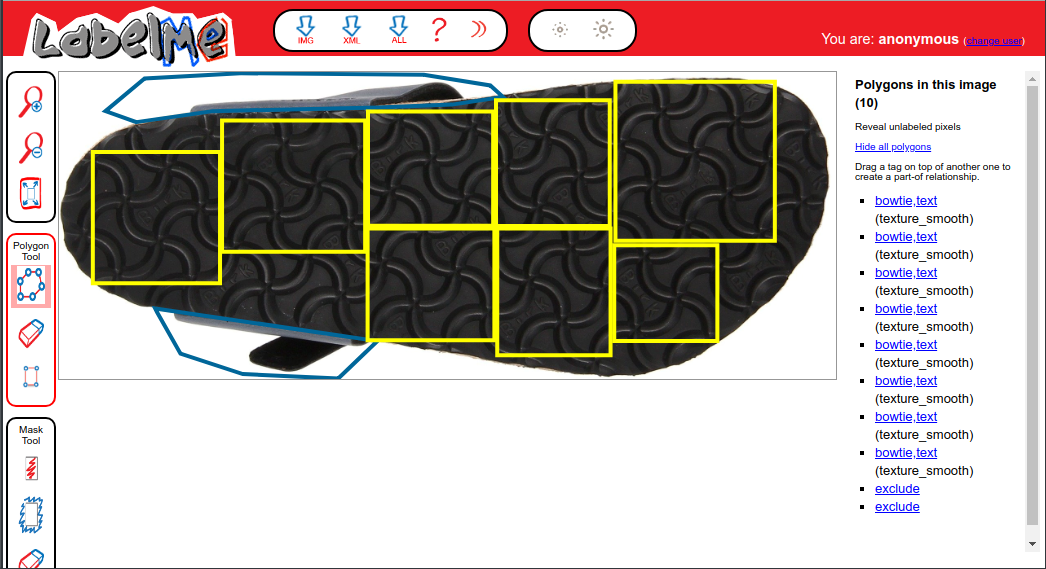
\includegraphics[width=\linewidth]{LabelMeScreenshot.png}
\captionof{figure}{LabelMe Tool \cite{LabelMe}}
\end{subfigure}
\end{minipage}
\vspace{1.35em}
\begin{itemize}\compresslist
    \item 24,000 multi-label images from 2,200 shoes
    \item Training set: 50\%, downsampled to get approximately equal numbers of each label
    \item Validation set: 25\%, used during training
    \item Test set: 25\%, used after training
\end{itemize}
}

%-------------------------------------------------------------------------------
%	RESULTS 1
%-------------------------------------------------------------------------------

\headerbox{Prediction Accuracy}{name=results,column=2,span=1,row=0,boxpadding=2mm}{
%\vspace{1em}
\begin{center}
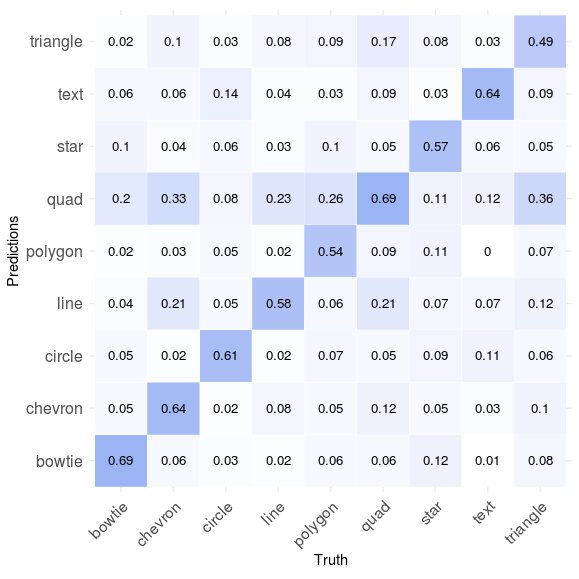
\includegraphics[width=0.68\linewidth]{ConfusionMatrix.png}\hspace{1mm}
\captionof{figure}{Percent of test images identified as containing a class with probability $\geq$ 0.2, after accounting for multiple labels}
\end{center}
}

%----------------------------------------------------------------------------------------
%	Applications
%----------------------------------------------------------------------------------------

\headerbox{Future Applications}{name=applications,column=2,span=1,below=results,boxpadding=2mm}{
\begin{itemize}
    \item Features for statistical models to assess match strength
    \item Speed up database searches
    \item Estimate frequency of class characteristics given information about local population
\end{itemize}
}

%----------------------------------------------------------------------------------------
%	REFERENCES
%----------------------------------------------------------------------------------------

\headerbox{References}{name=references, column=2, span=1, below=applications,above = bottom,boxpadding=2.5mm}{
\renewcommand{\section}[2]{} % Get rid of the default "References" section title
\nocite{*} % Insert publications even if they are not cited in the poster
\tiny{ % Reduce the font size in this block
%\begin{multicols}{2}
\bibliographystyle{unsrt}
\bibliography{Refs} % Use sample.bib as the bibliography file
%\end{multicols}
}}




%----------------------------------------------------------------------------------------
% \headerbox{foot}{name=foot,column=0, span=4, above=bottom}{
% abcdefghijklmnop}
%\cfoot{abcdddddddddddd}


\end{poster}
{\vspace*{0.05em}\tiny{This work was partially funded by CSAFE through Cooperative Agreement \# 70NANB15H176 between NIST and Iowa State University, which includes activities carried out at Carnegie Mellon University, University of California Irvine, and University of Virginia}
\end{document}
